\documentclass[14pt]{extbook}
\usepackage{multicol, enumerate, enumitem, hyperref, color, soul, setspace, parskip, fancyhdr} %General Packages
\usepackage{amssymb, amsthm, amsmath, bbm, latexsym, units, mathtools} %Math Packages
\everymath{\displaystyle} %All math in Display Style
% Packages with additional options
\usepackage[headsep=0.5cm,headheight=12pt, left=1 in,right= 1 in,top= 1 in,bottom= 1 in]{geometry}
\usepackage[usenames,dvipsnames]{xcolor}
\usepackage{dashrule}  % Package to use the command below to create lines between items
\newcommand{\litem}[1]{\item#1\hspace*{-1cm}\rule{\textwidth}{0.4pt}}
\pagestyle{fancy}
\lhead{Makeup Progress Quiz -1}
\chead{}
\rhead{Version B}
\lfoot{7547-2949}
\cfoot{}
\rfoot{Fall 2020}
\begin{document}

\begin{enumerate}
\litem{
Solve the rational equation below. Then, choose the interval(s) that the solution(s) belongs to.\[ \frac{81}{72x + 36} + 1 = \frac{81}{72x + 36} \]\begin{enumerate}[label=\Alph*.]
\item \( \text{All solutions lead to invalid or complex values in the equation.} \)
\item \( x \in [0.3,1.5] \)
\item \( x_1 \in [-0.6, -0.3] \text{ and } x_2 \in [-0.2,0.7] \)
\item \( x \in [-0.5,0.5] \)
\item \( x_1 \in [-0.6, -0.3] \text{ and } x_2 \in [-0.7,-0.3] \)

\end{enumerate} }
\litem{
Choose the graph of the equation below.\[ f(x) = \frac{1}{x + 1} - 3 \]\begin{enumerate}[label=\Alph*.]
\begin{multicols}{2}\item 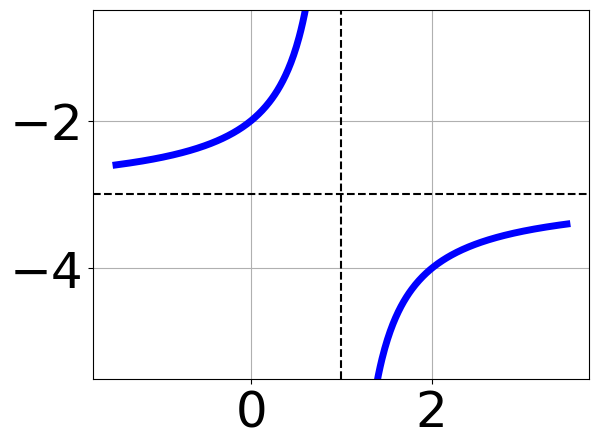
\includegraphics[width = 0.3\textwidth]{../Figures/rationalEquationToGraphCopyAB.png}\item 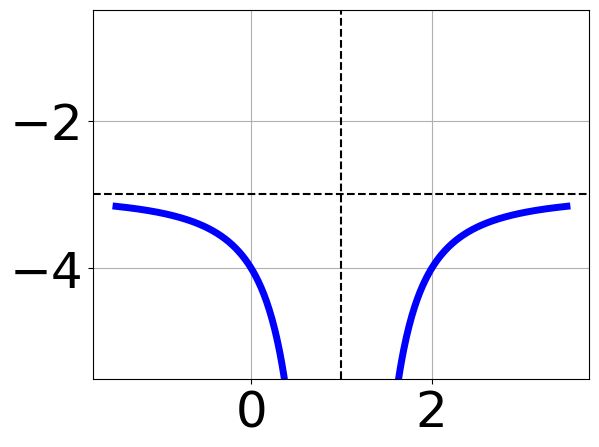
\includegraphics[width = 0.3\textwidth]{../Figures/rationalEquationToGraphCopyBB.png}\item 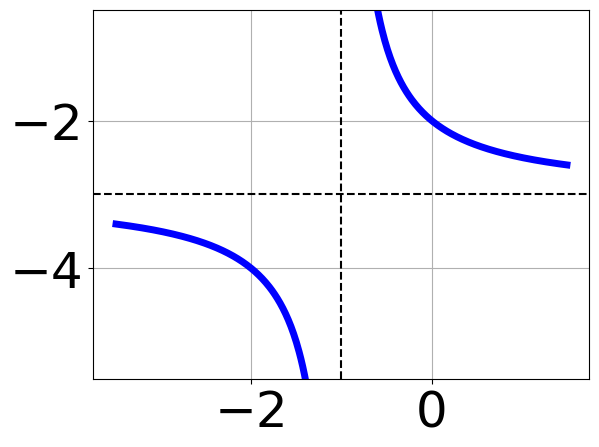
\includegraphics[width = 0.3\textwidth]{../Figures/rationalEquationToGraphCopyCB.png}\item 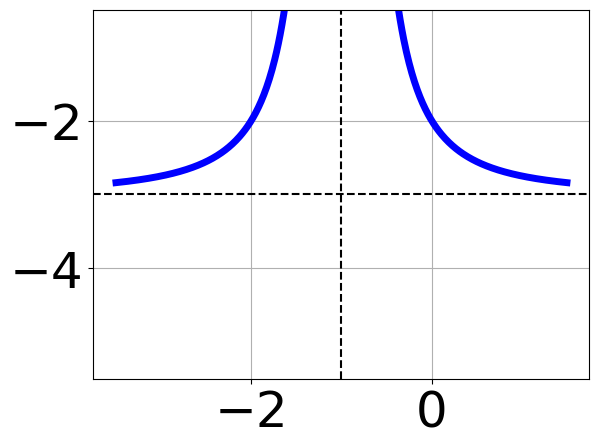
\includegraphics[width = 0.3\textwidth]{../Figures/rationalEquationToGraphCopyDB.png}\end{multicols}\item None of the above.
\end{enumerate} }
\litem{
Solve the rational equation below. Then, choose the interval(s) that the solution(s) belongs to.\[ \frac{24}{-96x + 24} + 1 = \frac{24}{-96x + 24} \]\begin{enumerate}[label=\Alph*.]
\item \( x \in [0.25,1.25] \)
\item \( x \in [-0.3,0.2] \)
\item \( x_1 \in [-0.3, 0.2] \text{ and } x_2 \in [0.25,1.25] \)
\item \( x_1 \in [-0.2, 0.7] \text{ and } x_2 \in [0.25,1.25] \)
\item \( \text{All solutions lead to invalid or complex values in the equation.} \)

\end{enumerate} }
\litem{
Determine the domain of the function below.\[ f(x) = \frac{3}{16x^{2} -32 x + 15} \]\begin{enumerate}[label=\Alph*.]
\item \( \text{All Real numbers except } x = a \text{ and } x = b, \text{ where } a \in [11.95, 12.24] \text{ and } b \in [19.77, 20.21] \)
\item \( \text{All Real numbers except } x = a, \text{ where } a \in [0.61, 0.94] \)
\item \( \text{All Real numbers.} \)
\item \( \text{All Real numbers except } x = a, \text{ where } a \in [11.95, 12.24] \)
\item \( \text{All Real numbers except } x = a \text{ and } x = b, \text{ where } a \in [0.61, 0.94] \text{ and } b \in [0.99, 1.38] \)

\end{enumerate} }
\litem{
Choose the equation of the function graphed below.
\begin{center}
    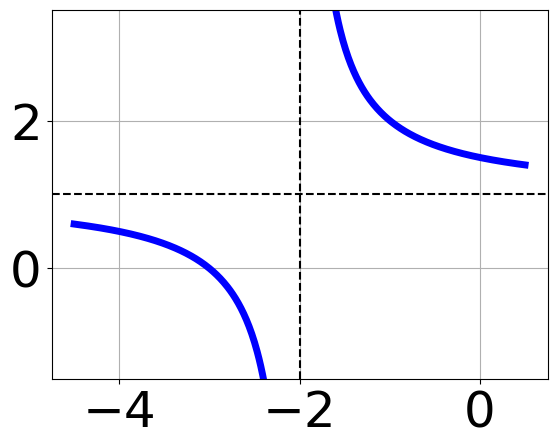
\includegraphics[width=0.5\textwidth]{../Figures/rationalGraphToEquationCopyB.png}
\end{center}
\begin{enumerate}[label=\Alph*.]
\item \( f(x) = \frac{1}{x - 2} + 2 \)
\item \( f(x) = \frac{1}{(x - 2)^2} + 2 \)
\item \( f(x) = \frac{-1}{(x + 2)^2} + 2 \)
\item \( f(x) = \frac{-1}{x + 2} + 2 \)
\item \( \text{None of the above} \)

\end{enumerate} }
\litem{
Determine the domain of the function below.\[ f(x) = \frac{5}{30x^{2} -11 x -30} \]\begin{enumerate}[label=\Alph*.]
\item \( \text{All Real numbers except } x = a, \text{ where } a \in [-2.5, -0.3] \)
\item \( \text{All Real numbers.} \)
\item \( \text{All Real numbers except } x = a, \text{ where } a \in [-31.8, -28.2] \)
\item \( \text{All Real numbers except } x = a \text{ and } x = b, \text{ where } a \in [-31.8, -28.2] \text{ and } b \in [29.8, 30.3] \)
\item \( \text{All Real numbers except } x = a \text{ and } x = b, \text{ where } a \in [-2.5, -0.3] \text{ and } b \in [0.1, 1.6] \)

\end{enumerate} }
\litem{
Choose the equation of the function graphed below.
\begin{center}
    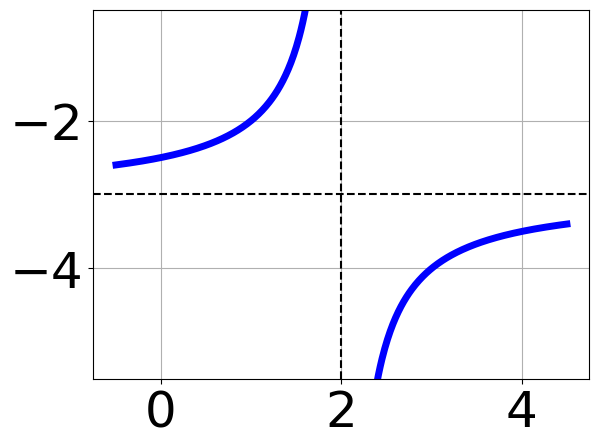
\includegraphics[width=0.5\textwidth]{../Figures/rationalGraphToEquationB.png}
\end{center}
\begin{enumerate}[label=\Alph*.]
\item \( f(x) = \frac{-1}{x - 2} - 3 \)
\item \( f(x) = \frac{1}{(x + 2)^2} - 3 \)
\item \( f(x) = \frac{1}{x + 2} - 3 \)
\item \( f(x) = \frac{-1}{(x - 2)^2} - 3 \)
\item \( \text{None of the above} \)

\end{enumerate} }
\litem{
Solve the rational equation below. Then, choose the interval(s) that the solution(s) belongs to.\[ \frac{-2x}{-2x + 5} + \frac{-3x^{2}}{14x^{2} -25 x -25} = \frac{5}{-7x -5} \]\begin{enumerate}[label=\Alph*.]
\item \( x_1 \in [0.22, 0.9] \text{ and } x_2 \in [-1.5,7.5] \)
\item \( x \in [-1.58,-0.08] \)
\item \( \text{All solutions lead to invalid or complex values in the equation.} \)
\item \( x \in [-2.96,-2.39] \)
\item \( x_1 \in [0.22, 0.9] \text{ and } x_2 \in [-7.67,-1.67] \)

\end{enumerate} }
\litem{
Choose the graph of the equation below.\[ f(x) = \frac{-1}{x + 3} + 3 \]\begin{enumerate}[label=\Alph*.]
\begin{multicols}{2}\item 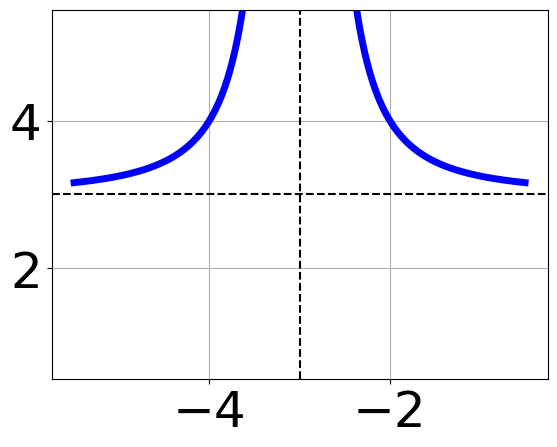
\includegraphics[width = 0.3\textwidth]{../Figures/rationalEquationToGraphAB.png}\item 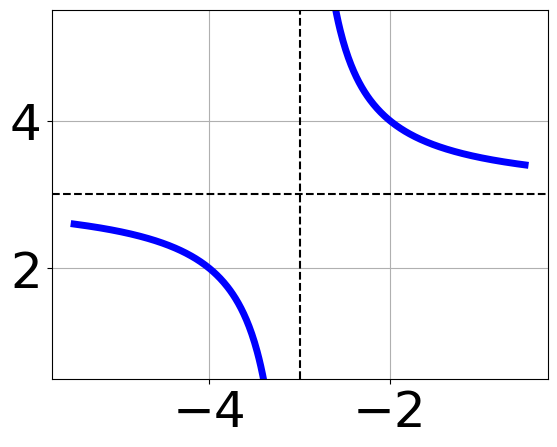
\includegraphics[width = 0.3\textwidth]{../Figures/rationalEquationToGraphBB.png}\item 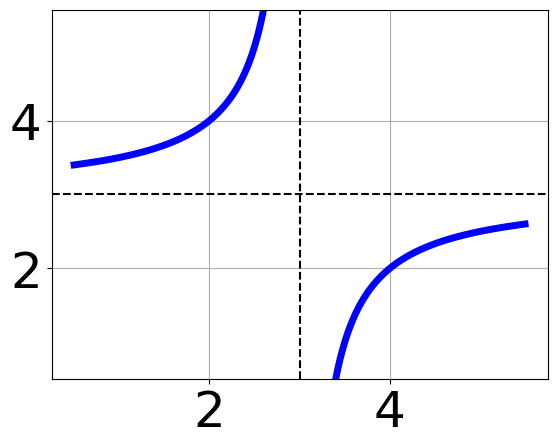
\includegraphics[width = 0.3\textwidth]{../Figures/rationalEquationToGraphCB.png}\item 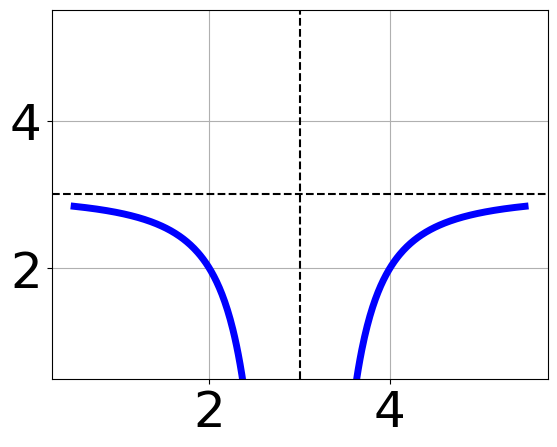
\includegraphics[width = 0.3\textwidth]{../Figures/rationalEquationToGraphDB.png}\end{multicols}\item None of the above.
\end{enumerate} }
\litem{
Solve the rational equation below. Then, choose the interval(s) that the solution(s) belongs to.\[ \frac{-6x}{6x + 6} + \frac{-4x^{2}}{12x^{2} +48 x + 36} = \frac{-4}{2x + 6} \]\begin{enumerate}[label=\Alph*.]
\item \( x_1 \in [-0.5, 2] \text{ and } x_2 \in [-3.42,-1.05] \)
\item \( x \in [-1.8,0.1] \)
\item \( \text{All solutions lead to invalid or complex values in the equation.} \)
\item \( x \in [-4.4,-2.9] \)
\item \( x_1 \in [-0.5, 2] \text{ and } x_2 \in [-1.21,-0.49] \)

\end{enumerate} }
\end{enumerate}

\end{document}